\genHeader
\hypertarget{installPlugin common}{} 
\subsection{Install our plugin for Eclipse}
 
\vspace{0.5cm}
 
\begin{stepbystep}

\item  Make sure that you have \textbf{Java~\JavaVersion{}} installed.
 
\item  Download and install Eclipse \EclipseVersion for modelling, which is called \textbf{Eclipse Modeling Tools} from \EclipseDownloadLink (\Cref{eclipseDownload}).\footnote{Please
note that you \emph{have to} install Eclipse Modelling Tools, or else some features won't work! Although different versions may support eMoflon, our tool is
currently tested only for \EclipseVersion~and Java \JavaVersion.} 

\begin{figure}[htbp]
	\centering
  	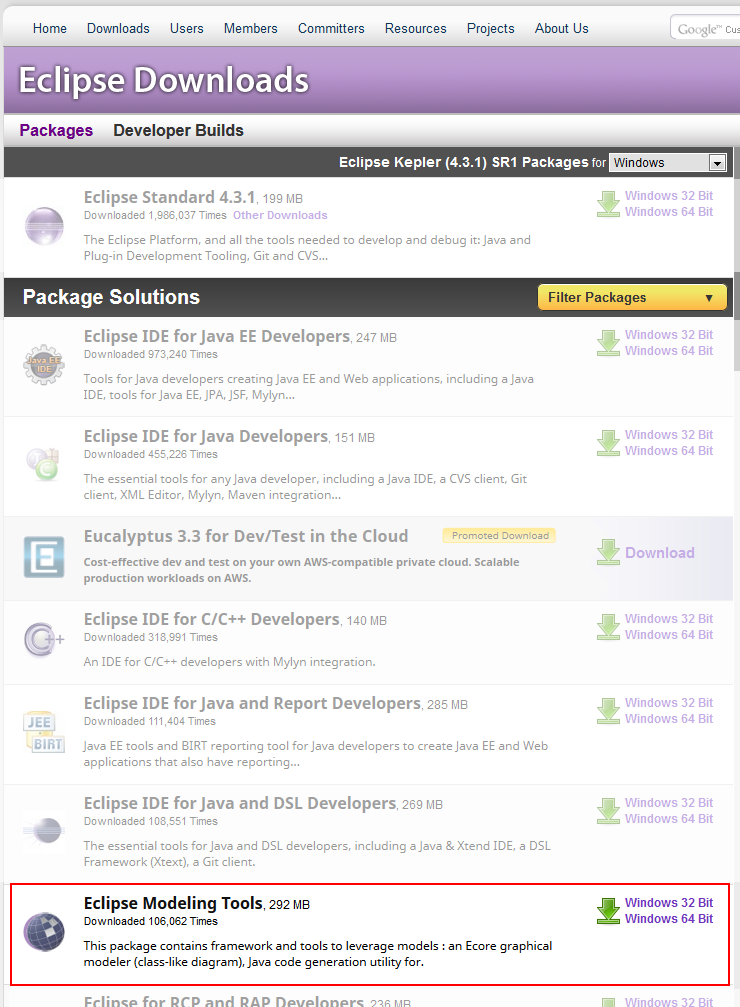
\includegraphics[width=0.55\textwidth]{../../org.moflon.doc.handbook.01_installation/1_installation/installPlugin/eclipseDownloadPage.png}
	\caption{Download \textbf{Eclipse Modeling Tools}}
	\label{eclipseDownload}
\end{figure}

\vspace{0.9cm}

\item  Install our Eclipse Plugin from the following update site\footnote{For a detailed tutorial on how to install Eclipse and Eclipse
Plugins please refer to \linkto{http://www.vogella.de/articles/Eclipse/article.html}}:\\ \eMoflonUpdateSite

\emph{Please note}: Calculating requirements and dependencies when
installing the plugin might take quite a while depending on your internet connection.

\emph{Hint:} To inform you about new updates, we maintain a Google group: \linkto{https://groups.google.com/forum/\#!forum/emoflon}
\end{stepbystep}
